\documentclass[10pt]{beamer}

%STANDARD PREAMBLE
%https://tex.stackexchange.com/questions/68821/is-it-possible-to-create-a-latex-preamble-header
\usepackage{/Users/mwojno01/Research/Learning/latex_preamble/beamer_preamble}

%
%% ALLOW FOR ITEMIZE ENVIRONMENTS WITH NO PRECEDING
% SPACING, IF DESIRED
% Reference: https://tex.stackexchange.com/questions/86054/how-to-remove-the-whitespace-before-itemize-enumerate
%\usepackage{enumitem}% http://ctan.org/pkg/enumitem 
\usepackage{paralist}

\title{Bayesian Linear Regression}

\begin{document}

\maketitle

\section{Why Bayesian Linear Regression?}

\begin{frame}{Why Bayes? (Linear Regression Version)}
\begin{itemize}
\item Provides a \textit{distribution} over regression lines
\item Automatically supports model selection / complexity control.
\item Easy access to nuanced inferential quantities.
\end{itemize}
	
\end{frame}


\subsection{Distribution over regression lines}
\begin{frame}{Bayesian Linear Regression}
\scriptsize

We learn a \textit{distribution} over regression lines.

\begin{center}
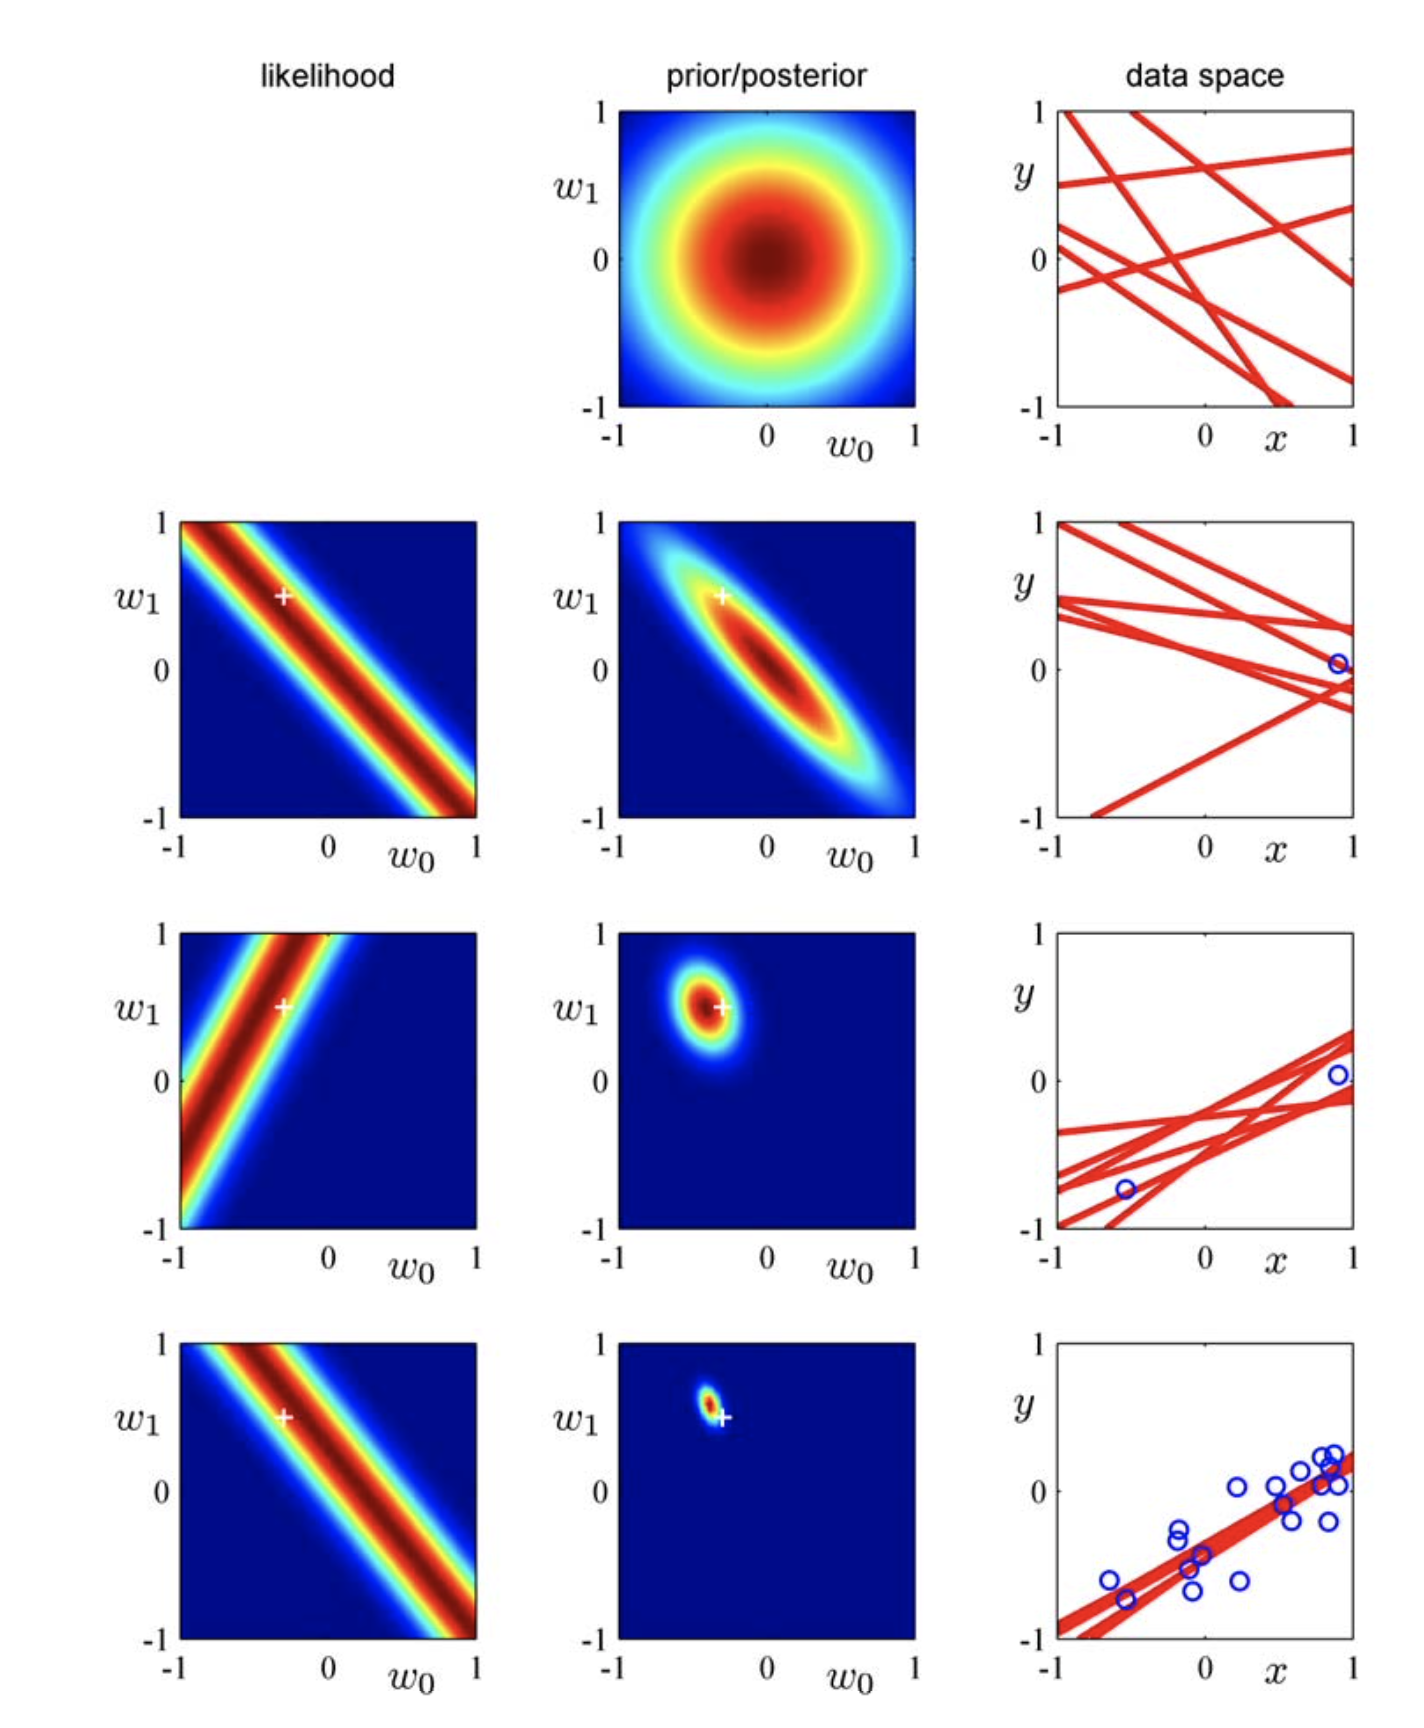
\includegraphics[width=.5\textwidth]{images/bishop_bayesian_regression}

Sequential Bayesian learning for a simple linear model.

\bottomtext{Image Credit: Bishop, C. M. (2006). Pattern recognition and machine learning. Springer.}
\end{center}




\end{frame}

\subsection{Automatic model selection}

\begin{frame}{Bayesian Occam's Razor}
\scriptsize

\textit{Remember this slide?}

\begin{center}
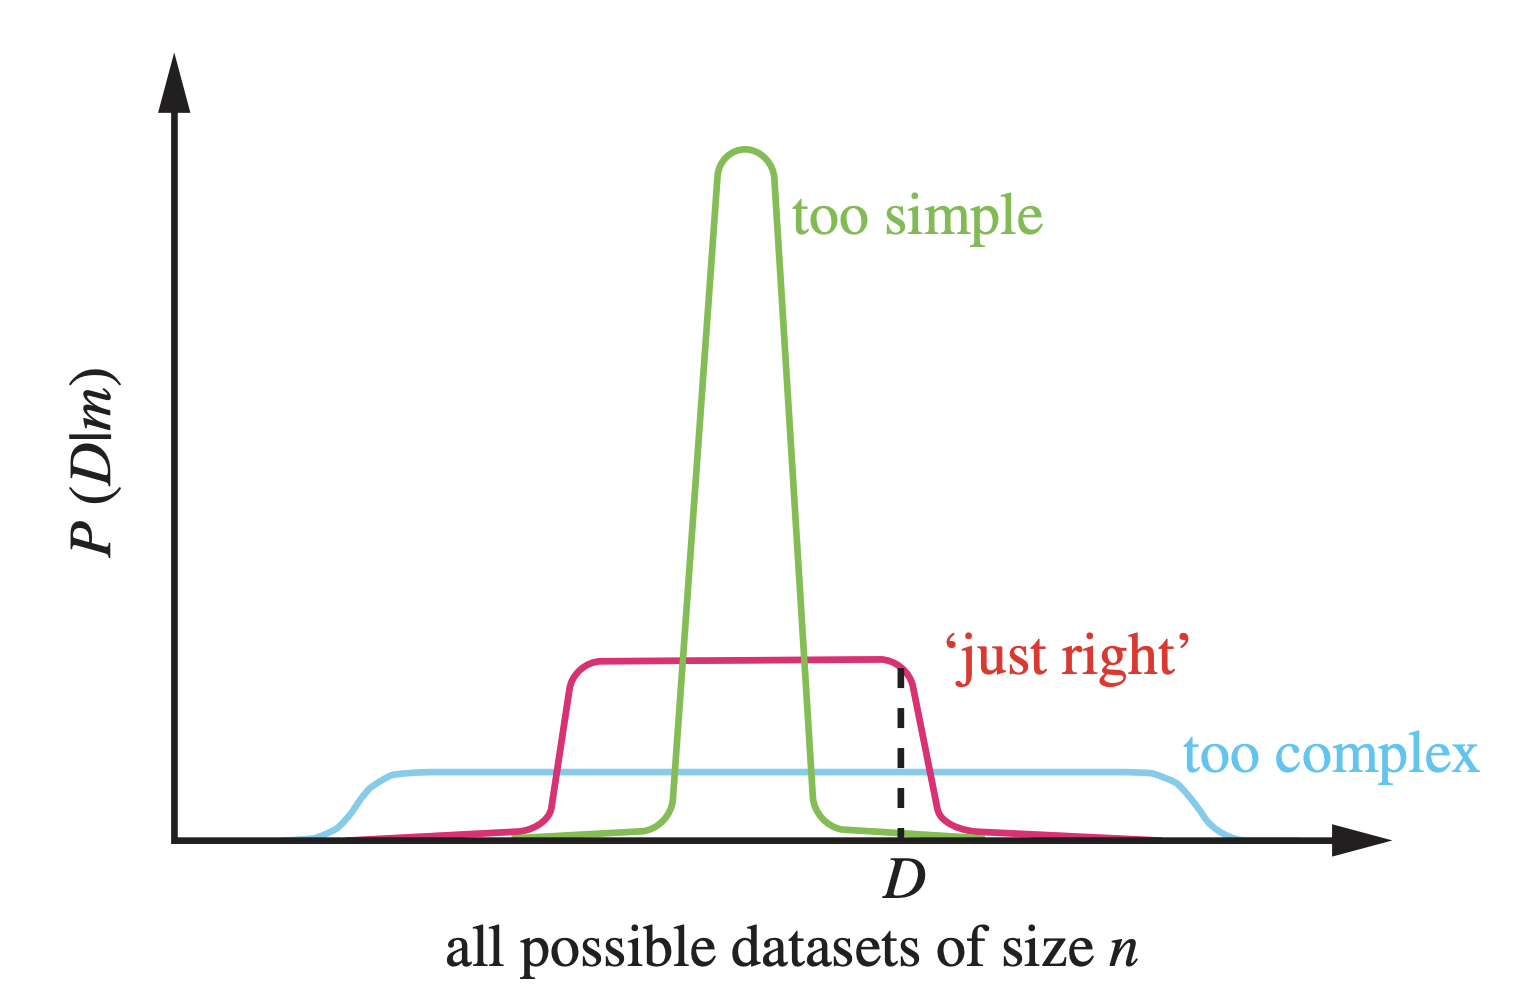
\includegraphics[width=.6\textwidth]{images/auto_occams_razor}
\end{center}
A \textit{complex} model (shown in blue) spreads its mass over many
more possible datasets, whereas a \textit{simple} model (shown in green) concentrates its mass on a smaller fraction of possible data.
Because probabilities have to sum to one, the complex model spreads its mass at the cost of not being able to model simple
datasets as well as a simple model—this normalization is what results in an automatic Occam razor. Given any particular
dataset, here indicated by the dotted line, we can use the marginal likelihood to reject both overly simple models, and overly
complex models. 


\bottomtext{Ghahramani, Z. (2013). Bayesian non-parametrics and the probabilistic approach to modelling. Philosophical Transactions of the Royal Society A: Mathematical, Physical and Engineering Sciences, 371(1984), 20110553.}
\end{frame}

\begin{frame}{Bayesian Occam's Razor}

{\scriptsize I generated $n=8$ data points from a \alert{cubic} distribution and used \texttt{NUTS} to fit Bayesian polynomials of various orders $p$.}

\vfill
    \begin{columns}
        \begin{column}{0.33\textwidth}
            %\centering %Uncomment this line for horizontal centering 
            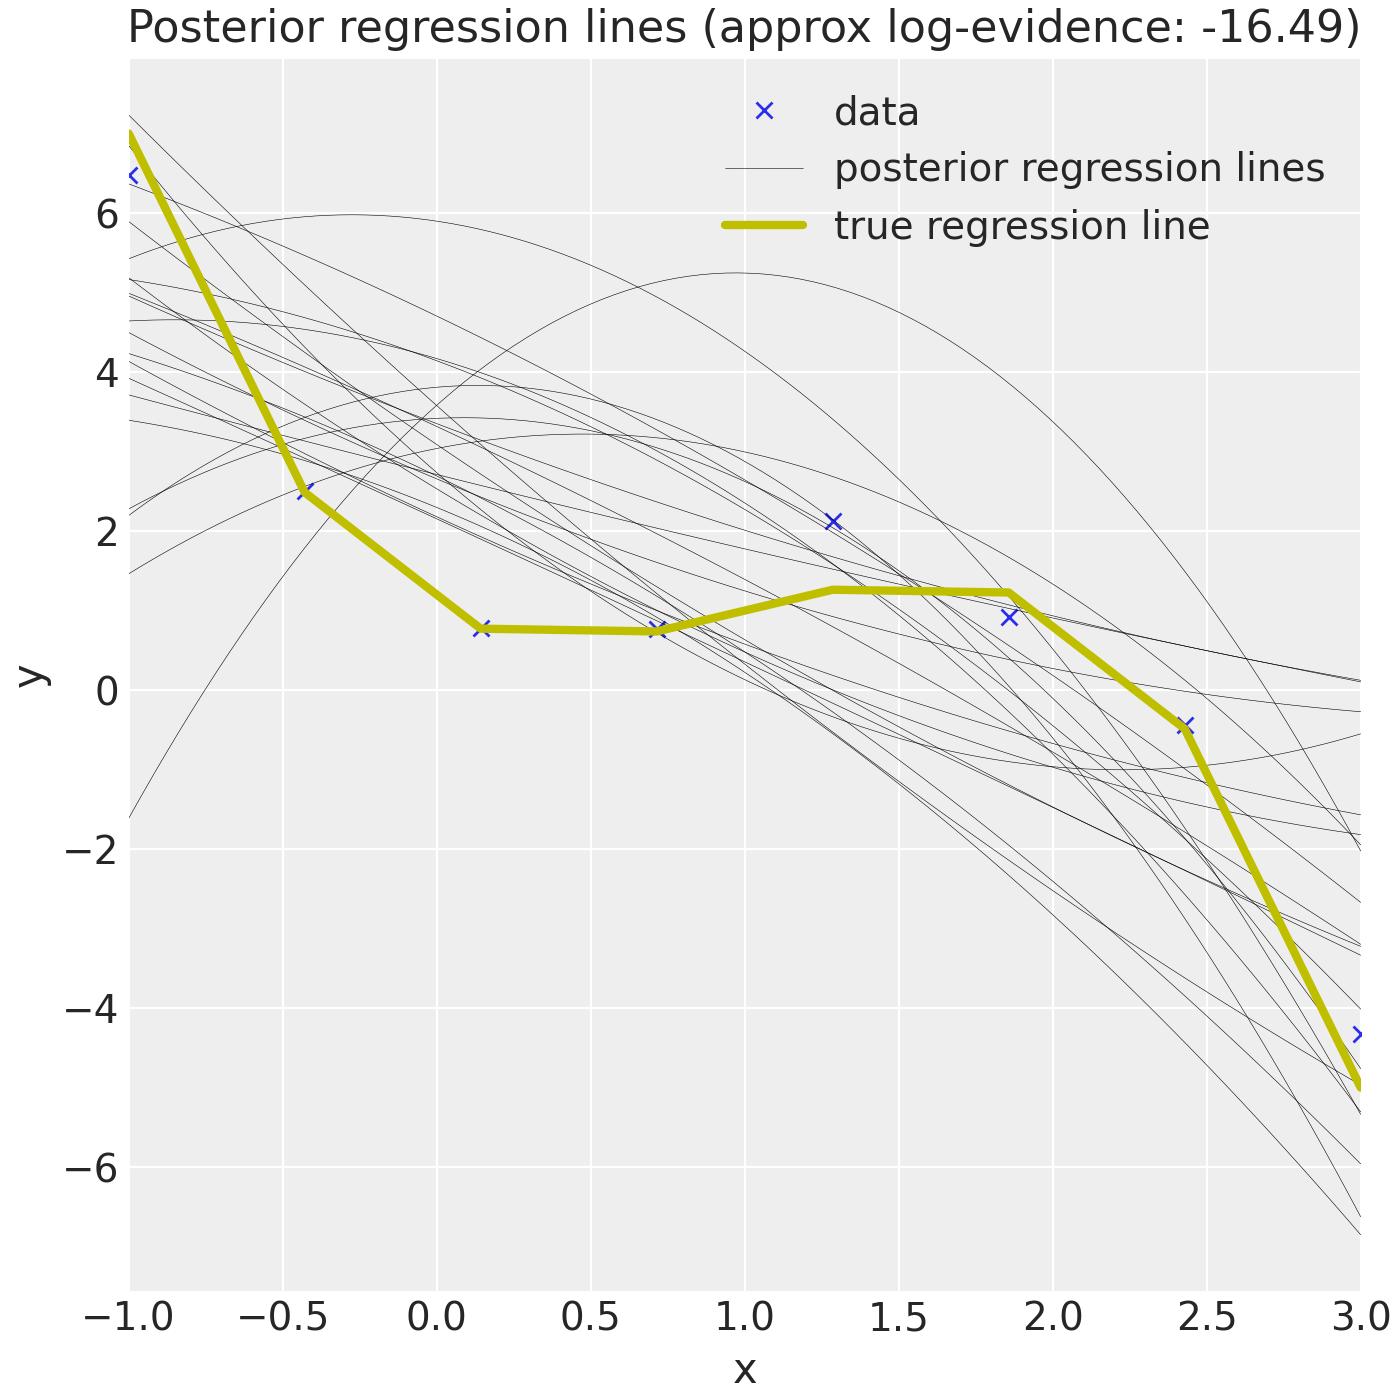
\includegraphics[width=\columnwidth]{images/bayesian_regression_quadratic_model}% \\
            
            Quadratic model ($p=2$)
        \end{column}
        \begin{column}{0.33\textwidth}
            %\centering %Uncomment this line for horizontal centering 
            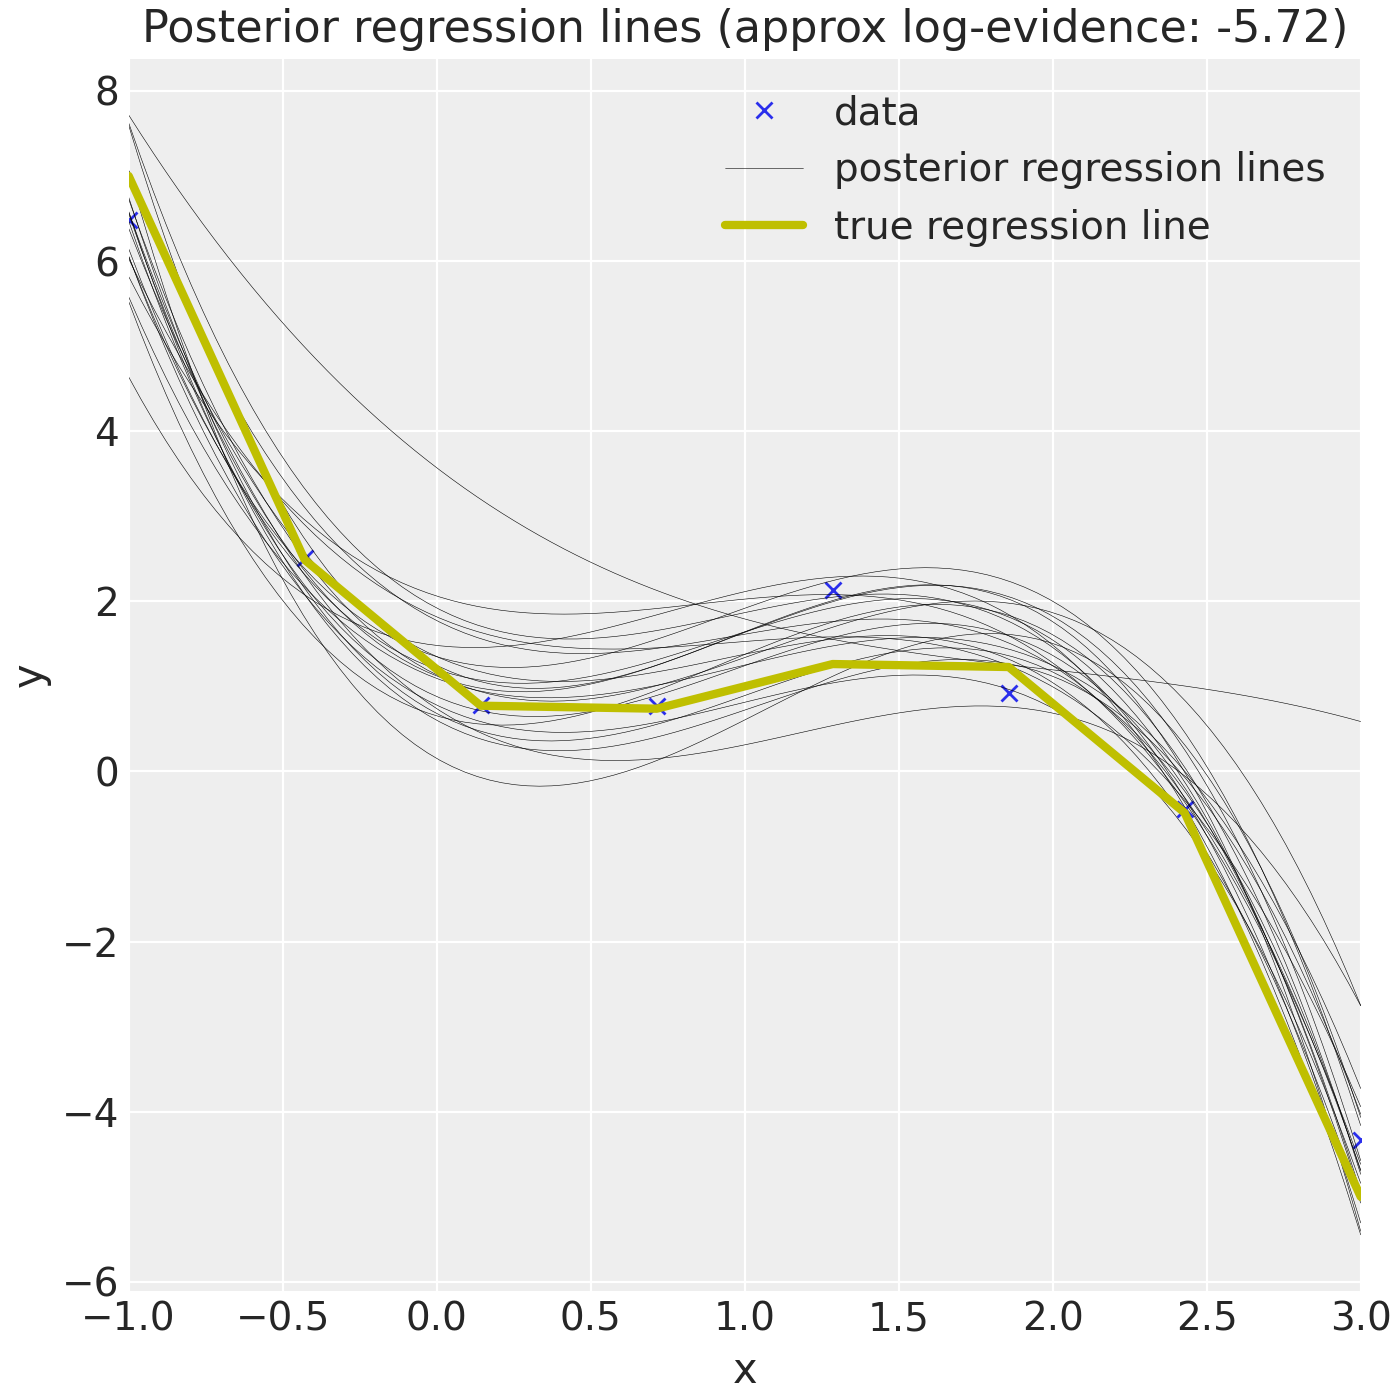
\includegraphics[width=\columnwidth]{images/bayesian_regression_cubic_model}%\\
            
            Cubic model ($p=3$)
        \end{column}
        \begin{column}{0.33\textwidth}
            %\centering %Uncomment this line for horizontal centering 
            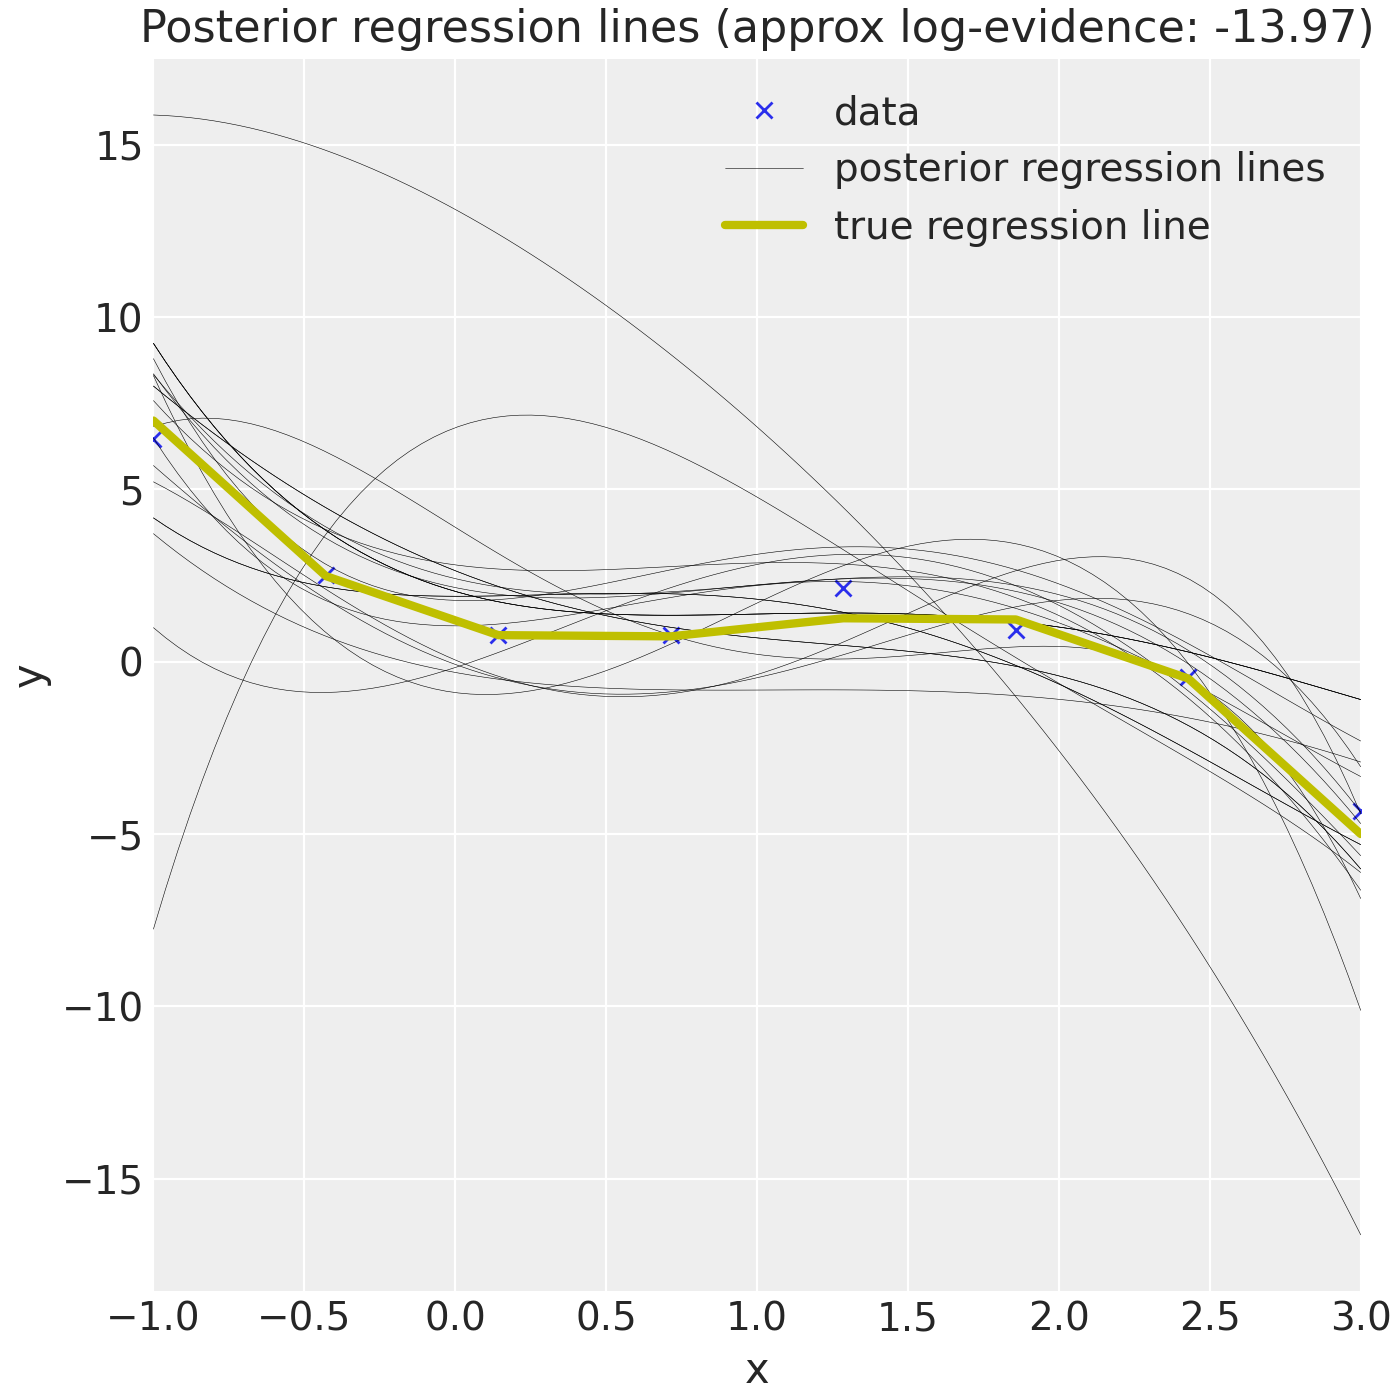
\includegraphics[width=\columnwidth]{images/bayesian_regression_fourth_order_model}%  \\
            
              Quartic model ($p=4$)
        \end{column}
    \end{columns}

\vfill 

{\scriptsize
\textbf{How does this align with the previous slide?} \pause 
\begin{itemize}
\item Bayesian model selection works well here!  The true (cubic) model has the highest evidence.  The evidence is lower for models that are underfit (quadratic) or overfit (quartic).
\item Posterior draws from the cubic model best match the true data generating process.
\item Maximum likelihood doesn't do this.  ML says: the higher the order, the \textit{better} the fit. 
\item The ranking of models by evidence matches what would be expected from the previous slide.

\end{itemize}
}

\end{frame}

\subsection{Easy access to nuanced inferential quantities}

\begin{frame}{Exercise Program Dataset \hfill \tiny (Hoff, \textit{A first course in Bayesian Statistical Methods}) }
	
\begin{center}
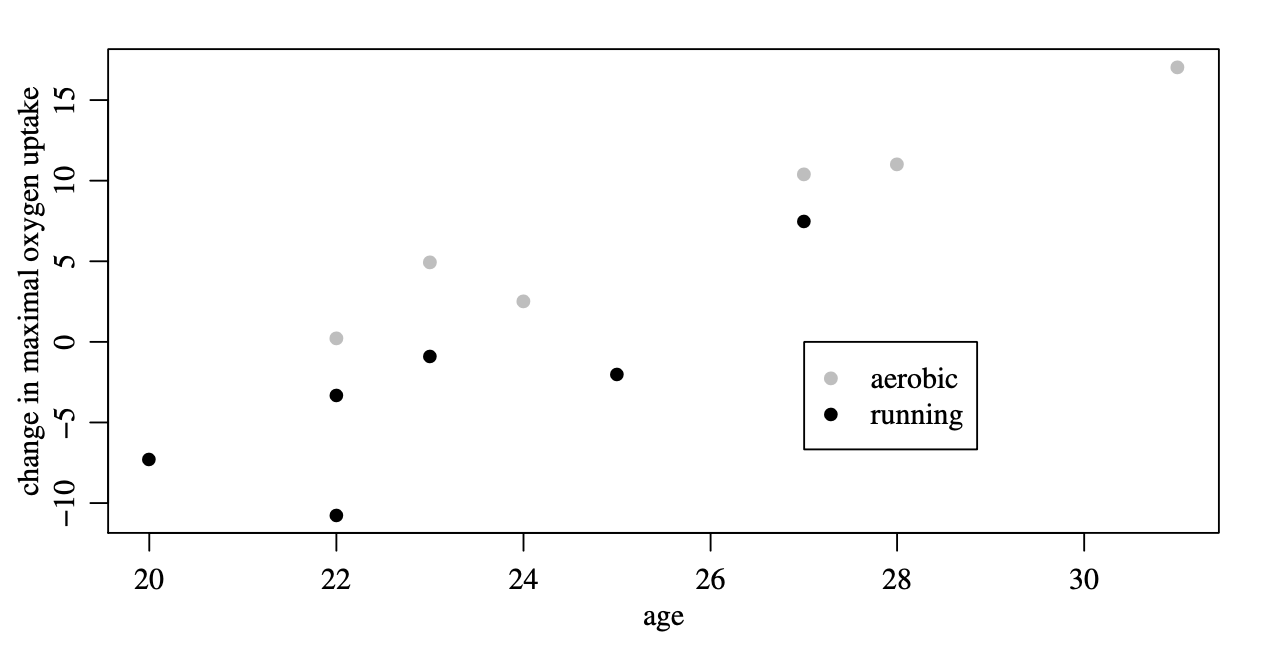
\includegraphics[width=.5\textwidth]{images/hoff_exercise_program_data}

\scriptsize Change in maximal $\text{O}_2$ uptake as a function of age and exercise program
\end{center}

{\normalsize \darkblue{Model}}
\scriptsize 
\begin{align*}
Y_i &= \beta_1 x_{i,1} + \beta_2 x_{i,2} + \beta_3 x_{i,3} + \beta_4 x_{i,4} + \epsilon_i, \; \text{where} \\
x_{i,1} &=1 \; \text{ for each subject $i$} \\
x_{i,2} &=0 \; \text{if subject $i$ is on the running program, 1 if on aerobic} \\
x_{i,2} &= \text{age of subject $i$} \\
x_{i,4} &= x_{i,2} \times x_{i,3}
\end{align*}

Under this model, the conditional expectations for $Y$ are:
\begin{align*}
\E[Y|\+x] &= \beta_1 + \beta_3 \times \text{age} \; \text{if $x_1 =0$, and} \\
\E[Y|\+x] &= (\beta_1 + \beta_2) + (\beta_3 + \beta_4) \times \text{age} \; \text{if $x_1 =1$} 
\end{align*}
%\bottomtext{Hoff, P. D. (2009). A first course in Bayesian statistical methods (Vol. 580). New York: Springer.}
\end{frame}

\begin{frame}{Frequentist Inference}
	
\begin{center}
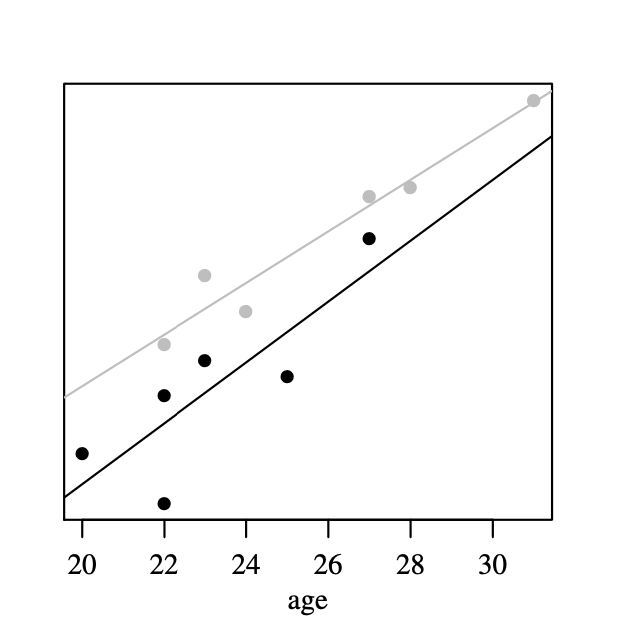
\includegraphics[width=.4\textwidth]{images/hoff_exercise_program_OLS_lines}

\scriptsize Maximum likelihood regression lines for the $\text{O}_2$ uptake data.
\end{center}

\begin{align*}
\widehat{\+\beta}_{\text{ML}} &= (-51.29, 13.11, 2.09, -.32)^T \\
\text{SE}(\widehat{\+\beta}_{\text{ML}} )& = (12.25, 15.76, 0.53, 0.65)^T 
\end{align*}

\scriptsize Comparing the values of $\widehat{\+\beta}_{\text{ML}}$ to their standard errors suggests the evidence for differences between exercise programs is not very strong.
\end{frame}


\begin{frame}{Bayesian Inference}
	
Bayesian inference agrees with the ML estimate, showing only weak evidence of a difference between exercise programs.

 \begin{figure}
\centering
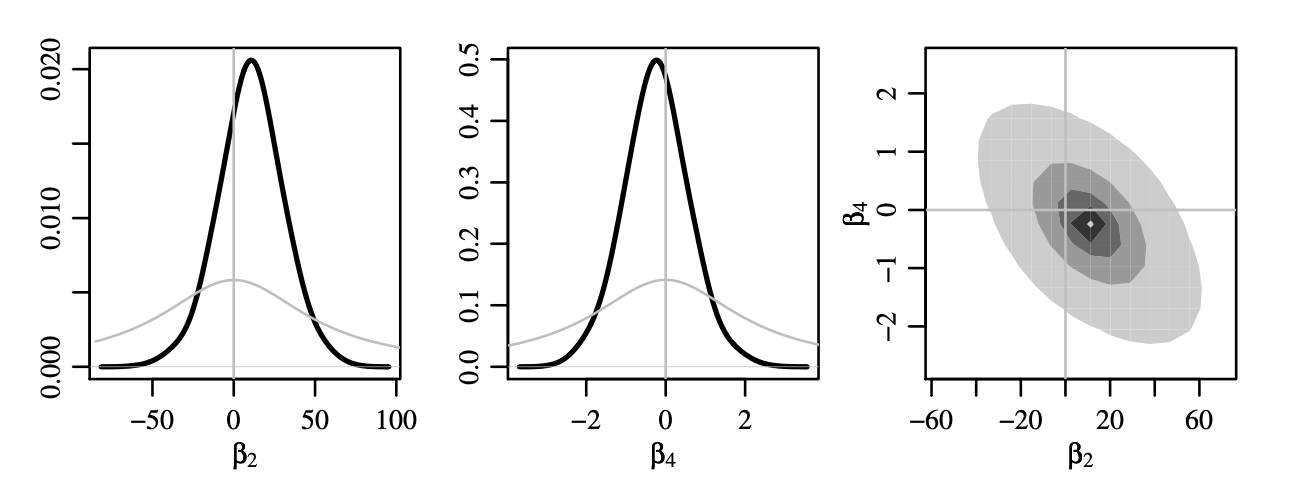
\includegraphics[width=.8\textwidth]{images/hoff_exercise_program_posteriors}
\caption{Posterior distributions for $\beta_2$ and $\beta_4$. The first two plots show the marginal prior distributions (grey) for comparison. The 95\% posterior intervals for $\beta_2$ and $\beta_4$ both contain 0.}
\end{figure}


\end{frame}

\begin{frame}{Bayesian Inference}
	
But the parameters by themselves don't tell the whole story. 

We can also look at the posterior distributions of $\beta_2 + \beta_4 x$ for each age x. 

 \begin{figure}
\centering
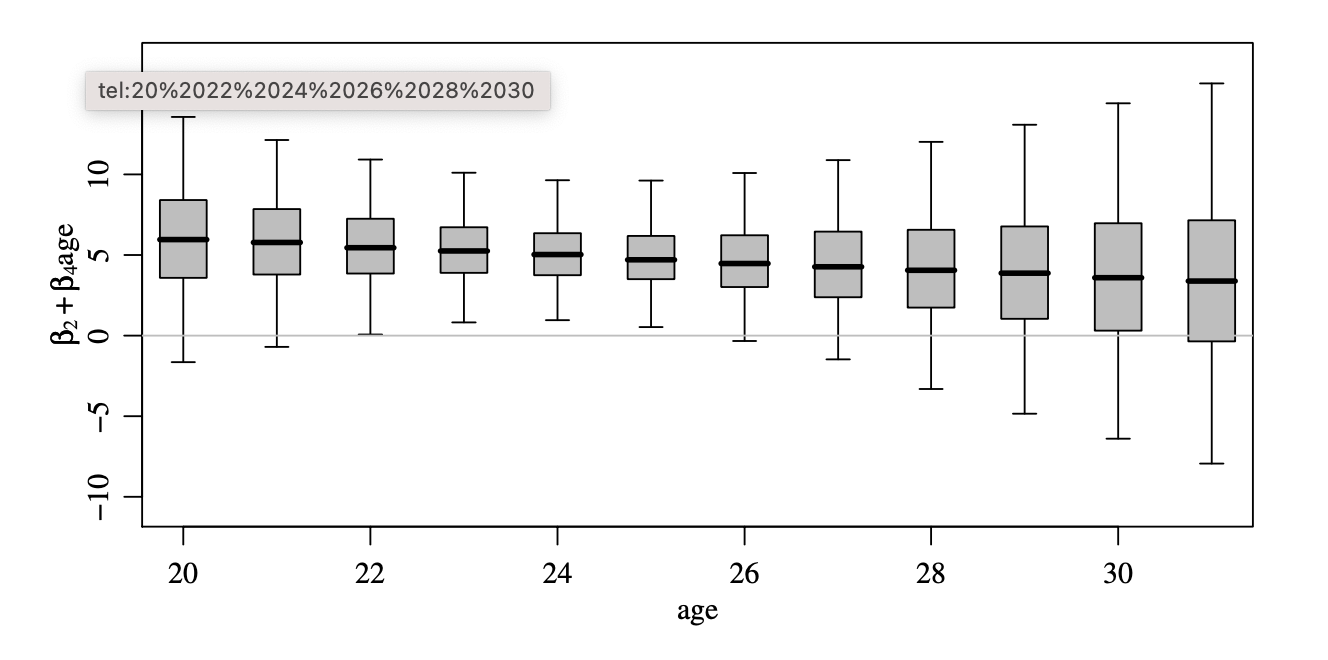
\includegraphics[width=.8\textwidth]{images/hoff_exercise_program_posteriors_by_age}
\caption{95\% confidence intervals for the difference in expected change scores between aerobics subjects and running subjects}
\end{figure}

This suggests reasonably strong evidence of a difference at young ages, and less evidence at older ones.

\end{frame}


%%%%%%%%%%%%%%%%%%%%%
\section{The model}

\begin{frame}{The model}

A basic Bayesian multiple linear regression model is given by

\vfill

\begin{align*}
\+\beta &\iid \N(\+\mu_0,  \+\Sigma_0) \\
\sigma^2 &\sim \InverseGamma (\frac{\nu_0}{2}, \frac{\nu_0}{2} \sigma_0^2) \\
y_{i} &\iid \N(\+\beta^T \+x_{i}, \sigma^2) \\
%\labelit \label{eqn:linear_regression}
\end{align*}

This model is conditionally conjugate. 
\end{frame}

\begin{frame}{Basis functions}
	
A linear regression model must be linear in its \textit{regression weights}, $\+\beta$, but need not be linear in its \textit{covariates} $\+x$.

More flexible models can be constructed by considering linear combinations of nonlinear functions of the covariates.



\begin{sblock}{Examples}
\pause \scriptsize 
For example, for a single covariate, the linear predictor $\eta_i := \E[y_i \cond \+\beta]$ could be given by
 \[ \eta_i  = \beta_0 + \sum_{m=1}^{M-1} \beta_{m} \phi_m(x_i)\]
 where
\begin{itemize}
\item polynomial basis functions take
 \[ \phi_m(x_i) = x_i^m \] 
 \hfill {\tiny (and such a model is known as \textit{polynomial regression})}
\item gaussian basis functions take
\[ \phi_m(x_i) = \exp \bigg\{ -\half \df{(x-\mu_m)^2}{s^2} \bigg\} \] 
\end{itemize}
\end{sblock}

\end{frame}

\begin{frame}{Prior specification}

A common choice of prior is obtained by setting the hyperparameters as follows:

\begin{sblock}{Prior on regression weights $\+\beta$}
\begin{itemize}
\item Standardize the covariates $\+x$.
\item Set $\+\mu_0 =\+0, \+\Sigma_0 = \+I$.
\end{itemize}
\end{sblock}

\begin{sblock}{Prior on observation noise $\sigma^2$}
The hyperparameters $(\sigma_0^2,  \nu_0)$ can be interpreted as the sample variance and sample size of prior observations.

\begin{itemize}
\item Set $\nu_0=1$.
\item Set $\sigma_0^2$ based on prior expectations.
\end{itemize}
\end{sblock}
\end{frame}

\begin{frame}{Weakly informative priors}

\scriptsize  Idea: if prior is not going to represent real prior information about the parameters, make it as minimally informative as possible.   Here are a couple of strategies:
\pause 
\vfill 
\begin{sblock}{The \textit{unit information prior} \hfill \tiny (Kass and Wasserman, 1995) }	
\scriptsize The precision of $\widehat{\+\beta}_{\text{ML}}$ is  $\Var^{-1} [\widehat{\+\beta}_{\text{ML}}] = (\+X^T\+X)/ \sigma^2$, and gives the amount of information in $n$ observations.  The unit information prior provides ``one $n$th" as much information 

\begin{itemize}
\item Set $\+\beta_0 = \widehat{\+\beta}_{\text{ML}}$.
\item Set $\+\Sigma_0^{-1} = (\+X^T\+X)/ (n\sigma^2)$
\end{itemize}

{\tiny Note: Strictly speaking, this is not a real \textit{prior} distribution.}
\end{sblock}

\pause 
\begin{sblock}{The $g$-prior \hfill \tiny (Zellner, 1986)}
Parameter estimation should be invariant to changes in scale of the regressors.  If $x_3 =$ age in years and $\wt{x}_3=$ age in months, then the posterior for $12 \times \wt{\beta}_3$ should be the same as the posterior for $\beta_3$. 

This condition is met if 
\begin{itemize}
\item Set $\+\beta_0 = \+0$.
\item Set $\+\Sigma_0^{-1} = k (\+X^T\+X)^{-1}$ for some $k$.
\end{itemize}

This prior specifies $k$ in terms of the error variance, $k=g \sigma^2$ for some $g$.  There are different methods for setting $g$, e.g. $g=n$.
\end{sblock}

\end{frame}


%%%%%%%%%%%%%%%%%%%%%
\section{Inference}


\end{document}